\documentclass{article}
\usepackage{graphicx}
\usepackage[labelfont=bf]{caption} 
\usepackage[numbers]{natbib}
\usepackage{amsmath}
\usepackage{float}
\usepackage{url}
\renewcommand{\refname}{\MakeUppercase{References}}
\title{\textbf{A New Qubits Mapping Mechanism for Multi-programming Quantum Computing}}
\author{{\Large Keshav Mishra\thanks{Permission to make digital or hard copies of part or all of this work for personal or
			classroom use is granted without fee provided that copies are not made or distributed
			for profit or commercial advantage and that copies bear this notice and the full citation
			on the first page. Copyrights for third-party components of this work must be honored.
			For all other uses, contact the owner/author(s).
			PACT ’20, October 3–7, 2020, Virtual Event, GA, USA
			© 2020 Copyright held by the owner/author(s).
			ACM ISBN 978-1-4503-8075-1/20/10.
			https://doi.org/10.1145/3410463.3414659}}\\
	{\normalsize Sys-Inventor Lab, SKLCA, ICT, CAS}\\
	{\normalsize *corresponding author (PI): lei.liu@zoho.com; liulei2010@ict.ac.cn}
}	

\date{}

\begin{document}
	
	\maketitle
	
	\begin{abstract}
		For a specific quantum chip, multi-programming helps to improve
		the overall throughput and resource utilization. However, previous
		solutions for mapping multiple programs often lead to resource
		under-utilization, high error rate, and low fidelity. In this paper, we
		propose a new approach to map concurrent quantum programs.
		Our approach has three critical components. The first one is the
		Community Detection Assisted Partition (CDAP) algorithm, which
		partitions physical qubits for concurrent quantum programs by con-
		sidering physical typology and the error rate, avoiding the waste
		of robust resources. The second one is the X-SWAP scheme that en-
		ables inter-program SWAPs and prioritizes SWAPs associated with
		critical gates to reduce the SWAP overheads. Finally, we propose a
		compilation task scheduler, which dynamically selects concurrent
		quantum programs to be compiled and executed together based
		on estimated fidelity for the best practice. We evaluate our work
		on publicly available quantum computer IBMQ16 and a simulated
		quantum chip IBMQ50. Our work outperforms the state-of-the-art
		work for multi-programming on fidelity and compilation overheads
		by 12.0\% and 11.6\%, respectively.
	\end{abstract}
	
	\section{Introduction}
	
	Quantum computer is stepping into our view. However, modern
	quantum chips belong to Noisy Intermediate-Scale Quantum (NISQ)
	category \cite{preskill2018quantum} - the qubits and the links between them are with
	variational reliability and are easily disturbed. The emergence of
	quantum cloud services enables users to access the quantum com-
	puters easily, but it also brings new challenges. As NISQ computers
	exhibit low fidelity, only programs with a few qubits can be exe-
	cuted reliably. Thus, NISQ computers tend to under-utilize their
	resources. Multi-programming can be an effective way. Although
	mapping multiple quantum programs onto a specific quantum chip
	improves the throughput, the activity of a program can negatively
	affect the reliability of co-located programs because of (i) limited
	number of qubits with high fidelity; (ii) cross-talk noise caused by
	simultaneously executed quantum gates; and (iii) long SWAP paths.
	In this paper, we propose solutions that improve the throughput
	and utilization of NISQ machines while reducing the negative im-
	pacts on the reliability of multi-programming NISQ computers. We
	find the previous qubits mapping policies have several shortcom-
	ings when handling multi-programming cases. (1) They often divide a large area of robust on-chip qubits into many small-scale seg-
	ments that cannot be mapped onto for other programs. On average,
	over 20\% of the robust qubits are wasted during the initial mapping.
	(2) When a specific quantum chip is partitioned for mapping mul-
	tiple quantum programs, post-compilation SWAP operations for
	each quantum program can be more, leading to an unpredictable
	impact for fidelity and reliability. For instance, additional SWAPs
	can be involved when two quantum programs with tens of CNOT
	gates are compiled together. (3) There is no ideal approach to select
	concurrent quantum programs for multi-programming on a specific
	quantum chip, leading to fidelity degradation and qubit resource
	under-utilization in many cases.
	Towards this end, we design a new qubits mapping mechanism,
	which has two key features. First, it partitions the physical qubits
	for concurrent quantum programs leveraging community detection
	techniques, avoiding the waste caused by the typology-unaware
	algorithms. It also provides a better initial-mapping, which reduces
	the SWAP overheads. Second, it is the First work that enables
	the inter-program SWAPs to solve the mapping problem in multi-
	programming cases that reduces the overall SWAP overheads. Our
	approach works well in practice. The experimental results show
	that our approach outperforms the latest solution \cite{das2019case} by 12.0\%
	on fidelity and 11.6\% on compilation overheads. Furthermore, we
	design a scheduler for selecting compilation tasks for the best prac-
	tice of multi-programming, avoiding the performance degradation
	caused by randomly selected workloads. The scheduler improves
	the throughput by 42.9\% and enhances the fidelity by 5.0\% over
	randomly selected workloads in our experiments, on average.
	
	\section{The Art of Our Design}
	
	\subsection{A new qubits mapping policy - CDAP}
	In this paper, we propose a new technology - Community Detec-
	tion Assisted Partitioning (CDAP) - to construct a hierarchy tree
	consisted of qubits for searching the robust qubits that are tightly
	connected for initial allocation. CDAP creates a hierarchy tree ac-
	cording to the coupling map and calibration data obtained from
	IBMQ API \cite{ibm2020quantum}. In the hierarchy tree, a leaf node denotes a spe-
	cific physical qubit; an internal node represents the union of its
	sub-nodes. Each node in the hierarchy tree is a candidate region
	for initial allocation. CDAP then iterates the hierarchy tree from
	bottom to top to find available regions for initial allocation
	quantum circuits are allocated by greedy policy to corresponding re-
	gions. The hierarchy tree is a profile of a quantum chip, which helps
	to locate reliable qubit resources on the quantum computer. The
	hierarchy tree construction algorithm is based on FN community
	detection algorithm, which clusters the physical qubits on a spe-
	cific quantum chip into communities. Qubits in a community have
	reliable and close interconnections.
	\begin{figure}[H]
		\centering
		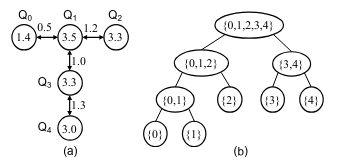
\includegraphics[width=0.7\textwidth]{figure_1.png}
		\caption[Bold]{\textbf{(a) Architecture of IBM Q London. The value in a
				node represents the readout error rate of the qubit, and the
				value on a link means the error rate of the CNOT operation.
				(b) The dendrogram, in which the values denote the index of
				the physical qubits.}}
		\label{fig:image1}
	\end{figure}
	
	
	
	In contrast, the links between communities have relatively low reliability.
	We explain why the hierarchy tree helps to select the initial allo-
	cation with an example in Figure 1. (i) $Q_0$ and $Q_1$ are firstly merged
	due to the link between them is with the lowest error rate. (ii) Then,
	$Q_2$ instead of $Q_3$ is merged into the community {0, 1}, though the
	link $Q_1$-$Q_3$ has lower CNOT error rate than $Q_1$-$Q_2$. This is because
	we tend to merge more inter-connected nodes into one community,
	avoiding the waste of robust physical qubits. Likewise, $Q_3$ and $Q_4$
	are merged. (iii) Finally, all qubits are merged as the root of the
	hierarchy tree as illustrated in Figure 1-(b). Our approach avoids the
	waste of robust resources caused by the typology-unaware greedy
	algorithm, and supports more quantum programs to be mapped on
	a specific quantum chip.
	
	
	\subsection{The design of inter-program SWAP - X-SWAP}
	Multi-programming brings new challenges for mapping transition.
	In this paper, we design the X-SWAP, including both inter and intra-
	program SWAP operations. In practice, the inter-program SWAP
	operation can be enabled when quantum programs are close to
	each other. The cost of inter-program SWAPs can be less than the
	cost in the cases where intra-program SWAPs are merely used.
	In our study, we find inter-program SWAPs take shortcuts. For
	instance, Figure 2-(a) shows two quantum programs are co-located
	(mapped) on a quantum chip with nine qubits. $q_1$ and $q_5$ are not
	mapped physically adjacent; SWAPs are required to satisfy their
	constraint to make CNOT $q_1$, $q_5$ executable. As illustrated in Figure
	2-(b), an inter-program SWAP, i.e., {$q_1$, $q_9$}, takes only one step (swap
	operation) to move $q_1$ and $q_5$ adjacent. In contrast, to achieve the
	same goal, previous intra-program scheme has to introduce three
	SWAPs, i.e., {$q_1$, $q_2$}, {$q_1$, $q_3$}, {$q_1$, $q_4$}. Briefly, enabling inter-program
	SWAPs could result in fewer SWAPs in the cases where multiple
	quantum programs are mapped as neighbors on a specific quantum
	chip, therefore reducing the SWAP overheads and benefiting the
	overall fidelity.
	
	
	
	
	\subsection{The design of the compilation task scheduler}
	
	Although there are some mapping mechanisms for concurrent quan-
	tum programs, selecting appropriate quantum programs to form
	a combination for the multi-programming workload is still a chal-
	lenging job. The workloads are now selected manually, which may
	cause the following defects. (1) Qubits on a specific quantum chip
	are under-utilized. (2) The program combinations formed by ran-
	domly selected programs may lead to a significant reduction in 
	\begin{figure}[H]
		\centering
		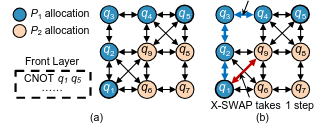
\includegraphics[width=0.7\textwidth]{figure_2.png}
		\caption{\textbf{(a)} $P$1 \textbf{and} $P$2 \textbf{are mapped on a quantum chip with
				9 qubits. The next gate to be solved is CNOT that involves}
			$q_1$ \textbf{and} $q_5$. \textbf{(b) X-SWAP scheme takes shortcuts to satisfy the
				constraint of CNOT} $q_1$, $q_5$.}
		\label{fig:image2}
	\end{figure}
	
	
	
	fidelity. (3) The results verification mechanism must be introduced
	to ensure the fidelity, which brings additional system modification
	overheads. To this end, we propose a design for the compilation task
	scheduler to select appropriate concurrent quantum programs for
	multi-programming. Our design focuses on selecting optimal quan-
	tum program combinations, maximizing the fidelity and resource
	utilization of the quantum chip. For each task in the scheduling
	queue, the scheduler checks whether other quantum programs in
	the queue can bring allowable fidelity reduction (e.g., the maximum
	reduction defined by the users) when they are co-located on the
	quantum chip with the current task. If so, they are mapped to the
	target quantum computer simultaneously for multi-programming.
	Otherwise, the task will be executed independently.
	
	
	\section{Evaluation}
	
	The baseline is the policy proposed in \cite{das2019case}, which generates ini-
	tial mapping for concurrent quantum programs with FRP strategy
	and generates mapping transition with the enhanced noise-aware
	SABRE. With our design, CDAP creates a reliable and close inter-
	connected initial mapping; X-SWAP reduces the compilation over-
	heads. CDAP and X-SWAP work together to benefit the perfor-
	mance - reducing the number of post-compilation gates by 11.6\%
	compared with baseline, and 8.6\% compared with SABRE \cite{li2019tackling}. The
	circuit depth is reduced by 16.0\% and 10.3\% compared with baseline
	and SABRE, respectively. The compilation task scheduler trades off
	between throughput and fidelity. It outperforms randomly selected
	workloads by 5.0\% on fidelity and improves the throughput of the
	quantum computer by 42.9\%. Moreover, our work exhibits scala-
	bility. It helps to improve the fidelity of the 2-program workloads
	on IBMQ16. For 4-program workloads on a quantum chip with 50
	qubits, it reduces the compilation overheads by 11.6\%
	
	\section*{ACKNOWLEDGMENTS}
	This project is supported by the National Key Research and De-
	velopment Program of China under Grant No. 2017YFB1001602
	and the NSF of China under Grant No. 61502452. Xinglei Dou is a
	student member in Sys-Inventor Lab supervised by Lei Liu.
	
	\bibliographystyle{plain}
	\bibliography{references}
\end{document}
